% Lecture 11
\subsection{Density Estimation \& GAMs}
\label{sub:densityestimationandgams}

\subsubsection{Density Estimation}
\label{ssub:densityestimation}

Standard problem in statistics and unsupervised learning: learn the distribution of the data. Classically: parametric familiy of densities $p(\theta),\>\>\theta\in\Theta$.

MLE: $\theta^* \overset{\text{max}}{\xrightarrow{}} \E \lbrack \ln p_\theta (\vx) \rbrack,\>\> \vx\sim p(\vx)$. In practice: expectation w.r.t. empirical distribution

\textbf{Prescribed models}: Ensure that $p_\theta$ defines a proper density $\int p_\theta(\vx)d\vx=1$

Trivial for models like exponential families. Impractical for complex models (Markov nets, DNNs). What are strategies for more complex models?

\textbf{Latent Variable Models}:

Classicaly: Define complex models via marginalization of a latent variable model

\tab $p_\theta(\vx)=\int p_\theta(\vx,\vz)d\vz$

EM algorithm (ELBO: evidence lower bound)

\tab $\log p_\theta(\vx)\geq \E_{q} \lbrack \log p_\theta (\vx,\vz) \rbrack +D_{\text{KL}}(q(\vz)||p_\theta(\vz)) \overset{\max\E}{\xleftarrow{}}\theta,q$

\tab optimal $q(\vx;\vz)=p_\theta(\vz|\vx)$ (posterior) not always tractable

\emph{Variational inference}: further approximation. Restrict to simpler families of distribution (weakening of ELBO), amortized inference $\Rightarrow$ variational auto-encoders.

\textbf{Unnormalized models}: Represent improper density functions:\\ \tab$\underbrace{\bar{p}_\theta(\vx)}_\text{represented}=\underbrace{c_\theta}_\text{unknown}\cdot \underbrace{p_\theta(\vx)}_\text{normalized}$

Can't use log-likelihood as scaling of $\bar{p}_\theta$ will cause unbounded likelihood. Alternative estimation method for unnormalized models?

\textbf{Score matching}: Is there an operator we can apply to $\bar{p}_\theta$ which does not depend on normalization? Score matching

\tab $\psi_\theta\coloneqq\nabla\log \bar{p}_\theta,\> \psi=\nabla \log p$

Minimize criterion: $J(\theta)=\E \lVert \psi_\theta - \psi \rVert^2$

Equivalently (eliminate $\psi$ using integration by parts):\\
\tab$J(\theta) \overset{\pm c}{=} \E \lbrack \sum_i \partial_i \psi_{\theta,i}-\frac{1}{2}\psi^2_{\theta,i}\rbrack$

Expectation approximated by sampling.

\textbf{Implicit Models}: Statistical models via: \emph{generating stochastic mechanism} or \emph{simulation process}.

\tab Latent code $\R^d\ni\vz\sim\pi(\vz),$ e.g. $\pit(\vz)=\cN(\mathbf{0},\vI)$\\
\tab parameterized mechanism $F_\theta: \R^d\xrightarrow{}\R^m$\\
\tab induced distribution $\R^m \ni \vx\sim p_\theta(\vx)$\\
\tab sampling is easy: random vector + forward propagation

\textbf{Noise Contrastive Estimation}: \emph{bootstrap} generative models via classification problems. Reduce density estimation to binary classification. Define probability ($p_n$: ``contrastive'' distribution: known distribution of negative samples, say ``everything but dogs'' and $p(\vx)$ is ``dogs'')

\tab $\Tilde{p} (\vx,y=1)=\frac{1}{2}p(\vx),\> \Tilde{p}(\vx,y=0)\frac{1}{2}p_n(\vx)$

Probabilistic classifier (induced by $\bar{p}_\theta$)

\tab $q_\theta = \frac{\alpha \bar{p}_theta}{\alpha \bar{p}_\theta + p_n},\> \alpha>0$.

Bayes optimal if $\alpha\bar{p}_\theta=p$. Minimize logistic loss with regard to $\theta$ and $\alpha>0$

This estimator is consistent! It is \emph{sometimes} statistically efficient, but generally \underline{no}.

\subsubsection{Generative Adversarial Models}
\label{ssub:gams}

Classification problem: distinguish between data \& model.

\tab $\Tilde{p}_\theta (\vx,y=1)=\frac{1}{2}p(\vx),\> \Tilde{p}_\theta(\vx,y=0)\frac{1}{2}p_n(\vx)$

Bayes optimal classifier: posterior $q_\theta=p/(p+p_\theta)$.

Train generator via minimizing the logistic likelihood:

\tab $\theta \overset{\min}{\xrightarrow{}}\ell^*(\theta)\coloneqq\E_{\Tilde{p}_\theta} \lbrack y \ln q_\theta(\vx) + (1-y)\ln(1-q_\theta(\vx))\rbrack$

Minimize Jensen-Shannon Divergence to get $\ell^*=\text{JS}(p,p_\theta)-\ln 2$

Generator's goal: generate samples that are \emph{indistinguishable from real data}, even for the best possible classifier. In general this in inaccessible, so we define a classficiation model:

\tab $q_\phi:\vx\mapsto\lbrack 0;1 \rbrack,\> \phi\in\Phi$.

Define objective via bound: \\
\tab$\ell^*(\theta)\geq \sup_{\phi\in\Phi}\ell(\theta,\phi),\> \ell(\theta,\phi)\coloneqq\E_{\Tilde{p}_\theta} \lbrack y\ln q_\phi(\vx) + (1-y)\ln(1-q_\phi)\vx))\rbrack$

Find best classifier within restricted family. Typically: $\Phi=$ weight space of DNN. Training objective is defined implicitly over $\sup$.

\textbf{Optimizing GANs}: Saddle point problem

\tab $\theta^*\coloneqq \argmin_{\theta\in\Theta} \{\sup_{\phi\in\Phi} \ell(\theta,\phi)\}$. Explicitly performing inner $\sup$ is impractical. 

SGD as a heuristic (may diverge!):

\tab $\theta^{t+1}=\theta^t-\eta\nabla_\theta\ell(\theta^t,\phi^t)$

\tab $\phi^{t+1}=\phi+\eta\nabla_\phi\ell(\theta^{t+1},\phi^t)$

\textbf{Evaluating GANs}: Conceptual question: how to measure \emph{quality} of implicit models? likelihood-based method not valid for implicit models. Trade-offs: noisy samples(e.g. blurry images), but adequate representation of variability. Faithful (as in: good looking) samples, but lack of representation (``mode dropping''). Which is better?


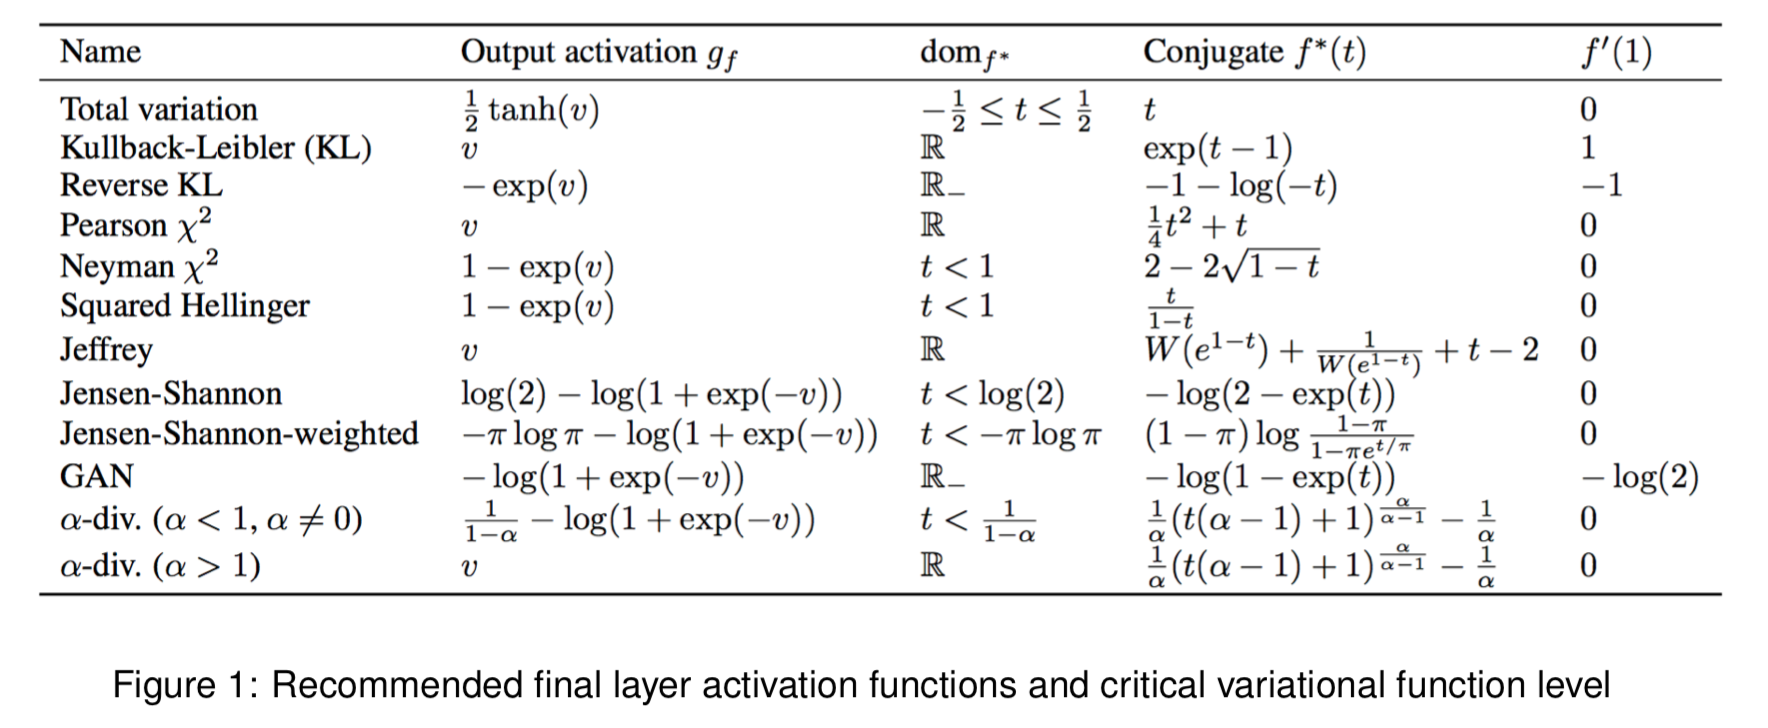
\includegraphics[scale=.25]{images/f-divergences.png}